%%%%%%%%%%%%%%%%%%%%%%%%%%%%%%%%%%%%%%%%%%%%%%%%%%%%%%%%%%%%%%%%%%%%%%%%
% INTRODUCTION DE L'ÉTUDE
%%%%%%%%%%%%%%%%%%%%%%%%%%%%%%%%%%%%%%%%%%%%%%%%%%%%%%%%%%%%%%%%%%%%%%%%

% ======================================================================
\section{Présentation du cadre d'étude}
% ======================================================================

% ----------------------------------------------------------------------
	\subsection{Le projet LSST}
% ----------------------------------------------------------------------

Le télescope LSST (\emph{Large Synoptic Survey Telescope}) est un projet mondial pour construire un télescope de surveillance continue du ciel. Il fait suite à des télescopes tels que SDSS ou Vista\footnote{Vista : (\emph{Visible and Infrared Survey Telescope for Astronomy}) télescope de l'ESO (European Southern Observatory) au Chili à partir de 2007.} qui ont pour but de rechercher des phénomènes astronomiques brusques et non prévisibles comme les supernovæ.

Le projet LSST est piloté par le laboratoire américain SLAC\footnote{SLAC : (\emph{Stanford Linear Accelerator Center}) Centre de l'accélérateur linéaire de Stanford, laboratoire de physique situé en Californie (États-Unis).}. Depuis son entrée dans le consortium en 2007, la collaboration LSST France compte aujourd'hui 8 laboratoires du CNRS provenant du département de recherche IN2P3 (Institut National de Physique Nucléaire et Physique des Particules). Ces laboratoires sont, par ordre alphabétique :
	\begin{itemize}
		\item \textbf{APC} (AstroParticules et Cosmologie) (Paris), pour la calibration et le contrôle commande de la caméra et le calcul ;
		\item \textbf{\CC} (Centre de Calcul IN2P3) (Lyon), calcul et gestion des données LSST ;
		\item \textbf{CPPM} (Centre de Physique des Particules de Marseille) (Marseille), pour le changeur de filtres et le calcul ;
		\item \textbf{LAL} (Laboratoire de l'Accélérateur Linéaire) (Orsay), pour l'électronique des CCD\footnote{CCD : (\emph{Charge-Coupled Device}) il s'agit d'un capteur photométrique permettant la prise d'images astronomiques.} ;
		\item \textbf{LMA} (Laboratoire des Matériaux Avancés) (Villeurbanne), pour mener la phase d'étude de faisabilité des filtres LSST ;
		\item \textbf{LPC} (Laboratoire de Physique Corpusculaire) (Clermont-Ferrand), pour le banc de test du système d'échange de filtres , et le calcul ;
		\item \textbf{LPNHE} (Laboratoire de Physique Nucléaire et de Hautes Énergies) (Paris), pour le carrousel de filtres, le banc de caractérisation de la caméra, l'électronique des CCD et le \emph{firmware} associé à l'électronique de contrôle et de lecture des CCD .
		\item \textbf{LPSC} (Laboratoire de physique subatomique et de cosmologie) (Grenoble), pour le banc de caractérisation de la caméra et le chargeur de filtres.
	\end{itemize}

	\begin{figure}[h!]
		\centering
		
\includegraphics[width=0.7\textwidth]{img/logo_LSST.png}
		\caption[Logo de LSST]{Logo de LSST.}
	\end{figure}

	\

Trois grands sujets d'étude ressortent de cette liste, la partie \emph{caméra} ayant rapport à la construction, aux tests et au développement de l'application de contrôle de la caméra, la partie dite \emph{calcul} ayant rapport aux développements d'applications, au traitement et stockage des données ainsi que le logiciel de calibration de la caméra, et finalement une partie dite \emph{science} s'occupant de l'interprétation des résultats.

% ----------------------------------------------------------------------
	\subsection{Le \emph{Stack} et \texttt{DC-2013}}
% ----------------------------------------------------------------------

Le \stack{} est le logiciel de traitement d'images du projet LSST. Contrairement à d'autres programmes jouant le même rôle sur d'autres télescope, celui-ci est pourvu d'un module de calibration le permettant de fonctionner avec des images en provenance de n'importe quel appareil. En effet ce module permet de transformer une image en une image calibré qui aura les mêmes propriété qu'importe sa provenance.

Le logiciel \stack{} est encore en cours de développement. Pour des raisons de gestion du projet, seul le personnel du laboratoire du SLAC est autorisé à participer à son développement, par conséquent très peu d'indications concernant la méthode de traitement d'image et le repérage des sources lumineuses sont disponibles.


		\subsubsection{La \emph{Data-Challange Summer 2013}}
% ^^^^^^^^^^^^^^^^^^^^^^^^^^^^^^^^^^^^^^^^^^^^^^^^^^^^^^^^^^^^^^^^^^^^^^

Durant l'été 2013, un test du \stack{} sur une partie des données de SDSS a été effectué en parallèle au centre de calcul de l'IN2P3 à Lyon (CC) et aux États-Unis. Pour cela les données brutes de SDSS de la \emph{stripe 82} ont été récupérées, puis traitées par le logiciel \stack.

Pour la partie française, 300 nœuds de calculs ont été mobilisés au CC de juin à octobre, pour analyser plus de 5\,\To{} de données. Le temps total de calcul est d'environ 300\,000 heures, ce qui représente 34 ans de calculs. On voit déjà l'importance de la parallélisation des calculs qui permet d'effectuer plusieurs calculs simultanément sur plusieurs nœuds.

La base de données générées est au format MySQL, fait 4,3\,\To{} (770\,\Go{} d'index (18\%) et 3,6\,\To{} de données (82\%), c'est environ 2 milliards de lignes par table, sachant qu'il y a 5 tables. L'indexation des données prend à elle seule 15 heures de calculs par table.

\ 

Cette expérience fut mené aussi aux États-Unis. Le nom donné à l'évènement fut \emph{Data-Challange Summer 2013} aussi abrégé en \DC{}.


		\subsubsection{Conclusion de la  \DC{}}
% ^^^^^^^^^^^^^^^^^^^^^^^^^^^^^^^^^^^^^^^^^^^^^^^^^^^^^^^^^^^^^^^^^^^^^^

Aucune analyse de la qualité des résultats ne fut effectuée en dehors d'un stage l'année passé, l'expérience reste donc plus une étude de faisabilité ainsi qu'un exploit technique. Il est maintenant nécessaire d'étudier les résultats du \stack{}, ceci permet de connaître mieux le logiciel ainsi que la qualité de ses résultats. Le stage que j'ai pu effectué l'an passé a permi une première analyse des résultats à l'aide d'un seul algorithme, mais les données nécessaire à ce traitement et les résultats obtenus sont stocker sous forme de fichiers texte.

\ 

Les calculs effectués aux États-Unis ainsi qu'en France n'ont pas porté sur le même jeu de données, seule une petite partie était commune pour vérifier que les résultats était semblable qu'importe la longitude. Le D\up{r} Phillipe \textsc{Gris} du LPC a effectuer cette comparaison de résultats, comme attendu la différences entre les résultats du \stack{} de part et d'autre de l'Atlantique sont nuls.


% ======================================================================
\section{Sujet d'étude}
% ======================================================================

Ce projet d'année est la suite d'un stage déjà effectué au LPC, ainsi le travail de préparation a déjà été effectué à cette occasion. L'aspcet théorique de certains algorithmes ont déjà été abordé, un modèle de base de donnée fut aussi étudié sur le papier. Ce projet est l'aboutissement de ce travail préparatoire, il s'agit donc d'approfondir les détails théoriques, d'implémenter ces algorithmes et un grand travail de test essentiellement sur la base de données ainsi que sur les différents algoritmes d'analyse. Ce travail de test permettra de déterminer la qualité des programmes d'analye de qualité pour en déduire lequel s'approprie le mieux à l'analyse des résultats du \stack.

% ----------------------------------------------------------------------
	\subsection{Stockage et accès aux données}
% ----------------------------------------------------------------------

Les données nécéssaires à l'analyse de qualité ne sont pas accessible facilement, ainsi un problème rencontré au cours du stage fut l'accès aux données du télescope SDSS. En effet une limitation de 10 requêtes par minutes est imposé par la base de données de SDSS, cela leur permet de garantir un accès public à tous, mais contraint l'exploitation en masse de résultats.

Les données générés par le \stack{} sont situés dans une multitude de fichiers au format \texttt{fits}. Le temps de lecture de ces fichiers est relativement lent surtout pour un traitement en masse de toute la portion de la \emph{stripe 82} analysée par le \CC.{}

\ 

Pour résoudre ces problèmes d'accès aux données amonts à l'analyse, il fut décidé pendant le stage de stocker ces données dans des fichiers textes. Ce choix est en parti dû à des contraintes techniques d'accès à une base de données ainsi que de temps de conception de celle-ci. Les résultats de l'analyse furent aussi stockés dans des fichiers textes au format \texttt{csv}. Ce format permet très simplement de stocker des données tabulaires.

\ 

Le problème que nous rencontrons avec ces fichiers texte est l'accès lent et difficile aux données. En effet nous ne disposons pas de la puissance d'une base de données relationnelles qui lié au langage SQL permet d'effectuer des recherches selon n'importe quel paramètres de manière aisé et rapide. De plus il est impératif d'avoir un produit robuste à la monté en charge, en effet seul 1\% des données totales furent analysé pendant le stage, et cela représenté déjà 2 millions de sources, donc de lignes, à sauvegardé. Ainsi le choix fut pris par l'équipe du LPC de stocker ces données dans uen base de données.


% ----------------------------------------------------------------------
	\subsection{Comparaison des données}
% ----------------------------------------------------------------------

La comparaison des résultats du \stack{} lors de la \DC{} et ceux de SDSS s'effectue par association. En effet à chaque élément découvert par SDSS on essaie d'y associer un élement traité par le \stack{}. Nous allons aussi effectuer un travil d'association ente les données du \stack{}. La première association (avec les données de SDSS) permet de vérifier la vraissemblance du logiciel de traitement d'images par rapport à des données dites de référence. La seconde association permet de comparer des résultats correspondant à des données sur la même portion de ciel, cela permet de vérifier la stabilité temporelle des données.

L'association s'effectue selon des critères à la fois astrométriques (les coordonnées de nos sources lumineuses), mais aussi photométrique (la luminosité de nos sources lumineuses). Par conséquent cela correspond à de la recherche de ressemblance ou en tout cas de la recherche de plus proche voisin.

\ 

La recherche de plus proche voisin est un sujet vaste qui s'applique aussi bien à des domaines comme la détection de forme, l'analyse de ressemblance mais aussi des détecteurs de collisions.

% ======================================================================
\section{Outils du projet}
% ======================================================================

% ----------------------------------------------------------------------
	\subsection{Outils de développement}
% ----------------------------------------------------------------------

Ce projet vivant au milieu du projet LSST, il est construit sur les mêmes bases. Le projet LSST impose l'utilisation du couple \Cpp{}/\Python{}.

			\paragraph{\Cpp}
Le langage \Cpp{} est un langage compilé, ce qui signifie que le code est d'abord converti en langage machine au cours de la compilation pour former un exécutable propre à une architecture (matériel et logiciel). L'intérêt réside dans la vitesse d'exécution, puisque l'exécutable est directement lu par la machine sans le moindre interpréteur.

Le \Cpp{} est un langage relativement bas niveau, cela signifie que la gestion de la mémoire est en bonne partie laissée au programmeur. Cela rend le développement plus long, et nécessite un certain nombre de connaissances pour éviter des erreurs de programmation.

Du fait de sa vitesse d'exécution le \Cpp{} est souvent utilisé pour des moteurs de calcul, ou des tâches sur un grand nombre de données.

			\paragraph{\Python}
Le langage \Python{} est un langage interprété, ce qui signifie qu'au moment de l'exécution, chaque ligne est traduite en langage machine avant d'être exécutée, et ce à chaque exécution d'un même script \Python. Les performances du \Python{} sont jusqu'à 100$\times$ moindre que celles du \Cpp{} comme le montre la figure~\ref{fig:cpp-py}.

	\begin{figure}
		\centering
		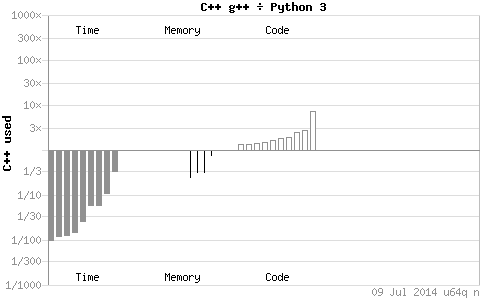
\includegraphics[width=0.8\textwidth]{img/cpp-py.png}
		\caption[Comparaison des performances entre \Cpp{} et \Python]{Cette étude compare les performances de \Python{} par rapport au \Cpp{} en effectuant le quotient \fraction{Performance \Cpp}{Performance \Python}, donc les résultats en dessous de 1 sont en faveur de \Cpp{}, ceux au dessus de 1 en faveur de \Python{}. Les tests s'effectuent en 3 catégories, temps d'exécution, utilisation de la mémoire et nombre de lignes de code. Chaque barre de l'histogramme dans une catégorie correspond à un algorithme (\emph{n-body}, \emph{mendelbrot}, \emph{binary-trees}, etc.). Source : \url{http://benchmarksgame.alioth.debian.org/}}
		\label{fig:cpp-py}
	\end{figure}

\Python{} est certes moins performant que \Cpp{}, mais il a l'avantage de facilité la programmation avec un nombre de lignes de code moins élevé, des fonctions haut niveau dans la bibliothèque standard et l'interpréteur qui permet un débogage plus rapide. \Python{} est donc privilégié pour la partie interface ainsi que l'ordonnancement des différentes tâches, laissant le cœur du calcul à \Cpp{}.

			\paragraph{MySQL}
La partie base de données implique le choix d'un système de gestion de base de données (SGBD), celui-ci est MySQL. Ce choix est la conclusion d'une étude sur les SGBD disposant d'une communauté importante. Pour de multiples raisons un logiciel libre est privilégié. Ainsi MySQL et PostgreSQL furent étudié, les deux SGBD disposant des plus grandes communautés. Le choix final se porta sur MySQL à cause d'une connaissance du logiciel par l'équipe devant utiliser les produits de projet à la fin de celui-ci.

MySQL est un projet apparu en 1995 et est devenu rapidement l'une des bases de données les plus utilisées aussi bien par le grand public que les professionnels où elle fait conccurence à \emph{Oracle} ou \emph{Microsoft SQL Server}.

L'aspect base de données ne sera pas la partie la plus détaillée de ce rapport puisqu'il ne s'agit pas de l'aspect principal de ce projet. L'utilisation de NoSQL\footnote{NoSQL : (\emph{Not Only SQL}) est un paradigme de base de données ne faisant pas intervenir seulement SQL.} n'a pas été envisagé par manque de connaissances sur le sujet.


% ----------------------------------------------------------------------
	\subsection{Outils de gestion du projet}
% ----------------------------------------------------------------------

%	\begin{ganttchart}{0}{13}
%		\gantttitle{2014}{8}
%		\gantttitle{2015}{6}\\
%		\gantttitlelist{9,...,12,1,2,3}{2} \\
%		
%		\ganttgroup{Aspect théorique}{0}{6} \\
%		\ganttbar{Recherche de l'existant}{2}{4} \\
%		\ganttbar{Cahier des charges}{0}{4} \\
%		\ganttbar{Implémentation}{2}{6} \\
%		\ganttbar{Recherche de modèle BDD}{2}{6} \\
%		
%		\ganttgroup{Mise en production}{7}{12} \\
%		\ganttbar{Débugage}{6}{10} \\
%		\ganttbar{Tests}{6}{10} \\
%		\ganttbar{Analyse des résultats}{10}{12} \\
%	\end{ganttchart}

%\newgantttimeslotformat{stardate}{%
%\def\decomposestardate##1.##2\relax{%
%\def\stardateyear{##1}\def\stardateday{##2}%
%}%
%\decomposestardate#1\relax%
%\pgfcalendardatetojulian{\stardateyear-01-01}{#2}%
%\advance#2 by-1\relax%
%\advance#2 by\stardateday\relax%
%}

%\begin{ganttchart}[hgrid, vgrid, time slot format=stardate]{2014.9.1}{2015.3.15}
%\gantttitlecalendar{year, month=name} \\
%\end{ganttchart}
